\section{Introduction}
Computer scientists are used to deal with discrete systems, i.e. systems whose evolution can be described by a sequence of discrete state changes. A widespread example is the program analysis: during the execution of a program, the system is abstracted into a state machine whose states changes every time an instruction is executed.
In the past decade, due to the increasing usage of digital controllers, the interest in safety verification has risen. Especially complex and critical systems such as planes or nuclear reactors, which are controlled by digital systems require extensive safety verification.. The states of these systems are described not only by a discrete one (flying, launching, exploding...), but also by physical variables (velocity, temperature...), which evolve continuously over the time. Such systems, with continuous and discrete components are called hybrid systems. These systems are omnipresent, whenever a digital controller interacts with continuous quantities there is a hybrid system, even for devices as simple as a digitally controlled thermostat with the temperature.

For verification purposes, these systems are abstracted into hybrid automata, which is a common model for hybrid systems~\cite{colas}. Example~\ref{exp_thermostat} describes a thermostat and the associated automaton.

\begin{example} A thermostat controls a heater in a room. Let $T$ be the temperature in the room, the thermostat is programmed to keep the temperature between $17$\textdegree C and $23$\textdegree C.
The heater can be in two states:
\begin{itemize}
\item ON: the temperature in the room increases according a linear differential equation. If the temperature is above $22$\textdegree C and before it reaches $23$\textdegree C, the heater is turned off.
\item OFF: the temperature in the room decreases according a linear differential equation. If the temperature is below $18$\textdegree C and before it reaches $17$\textdegree C, the heater is turned on.
\end{itemize}
The thermostat can be described with the state of the heater, discrete, and the temperature of the room, continuous, it is a hybrid system.


The associated hybrid automaton has the same discrete states as the system: ON and OFF. There will be only one continuous variable: the temperature. The evolution of the temperature is controlled by the current discrete stateand the change of the discrete states is connected to the current temperature. Figure~\ref{fig_thermostat} shows the evolution of the temperature for a system initialized with a heater on and $20$\textdegree C and the resulting hybrid automata.

\begin{figure}

 \begin{tikzpicture}[scale=0.5]
  \thermostatcon{0}{0};
 \end{tikzpicture}
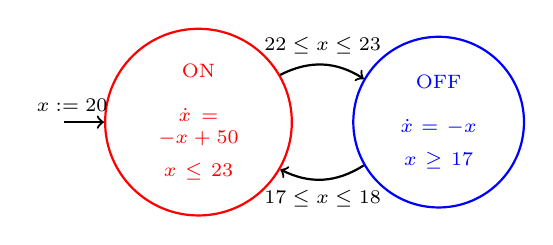
\begin{tikzpicture}[scale=0.61]
  \node[draw, circle, text width = 1.4cm, text centered, thick,color=red] (l1) at (0,0) {\scriptsize{ON\\ \ \\$\dot{x}=-x+50$\\ $x\leq 23$}};
  \node[draw, circle, text width = 1.4cm, text centered, color=blue, thick] (l2) at (5,0) {\scriptsize{OFF\\ \ \\$\dot{x}=-x$\\ $x\geq 17$}};
  \path[thick,->] (l1) edge[bend left] node[above] {\scriptsize{$22\leq x\leq 23$}} (l2);
  \path[thick,->] (l2) edge[bend left] node[below] {\scriptsize{$17\leq x\leq 18$}} (l1);
  \node (dummy) at (-3,0) {};
  \path[thick,->] (dummy) edge node[pos=0.2, above] {\scriptsize{$x:=20$}} (l1);
 \end{tikzpicture}
\caption{On the left: the evolution of the temperature for the given thermostat initialized on the state (ON,$20$\textdegree C). On the right: the corresponding hybrid automata. Illustrations taken from Erika \'Abr\'aham's presentation in Genoa, Octorber 2015.}
\label{fig_thermostat}
\end{figure}

\label{exp_thermostat}
\end{example}

A hybrid automaton is described by a finite set of discrete states and a finite set of continuous variables. The evolution of the variables is determined by the current discrete state. The current state of the system is defined by the discrete state it is in and by the current value of the continuous variables. A transition between two discrete states can be done under certain conditions (called a guard) over the variables. To stay in a given discrete state, a condition has to be satisfied (called the invariant of the discrete state). A transition can reassign the variables. All these parts can be seen in Figure~\ref{fig_thermostat}.



\begin{table}
\centering
\begin{tabular}{| c | c | c | c | c |}
	\hline	
	Sub- & derivative & conditions & bounded  & unbounded \\
	classes & & & reachability & reachability \\ \hline
	TA & $\dot x=1$ & $x\overset{?}{=}c$ & \textcolor{green}{\checkmark} &\textcolor{green}{\checkmark} \\ \hline
	& & $x\overset{?}{\in} [c_1;c_2]$ & &   \\	
   	IRA & $\dot x\in [c_1;c_2]$ & jump must reset &\textcolor{green}{\checkmark} &\textcolor{green}{\checkmark} \\ 
   	& & $x$ when $\dot x$ changes & &\\ \hline
   	RA & $\dot x\in [c_1;c_2]$ & $x\overset{?}{\in} [c_1;c_2]$ &\textcolor{green}{\checkmark} &\textcolor{red}{X} \\ \hline
   	LHA I & $\dot x=c$ & $x\overset{?}{=}g_{linear}$ &\textcolor{green}{\checkmark} &\textcolor{red}{X} \\ \hline
   	LHA II & $\dot x=f_{linear}$ & $x\overset{?}{=}g_{linear}$ &\textcolor{red}{X} &\textcolor{red}{X} \\ \hline
   	HA  & $\dot x=f$ & $\dot x=g$ &\textcolor{red}{X} &\textcolor{red}{X} \\ \hline
\end{tabular}
\vspace*{0.3cm}
\label{tab_complexity}
\caption{Decidability results for subclasses of automata. $c$, $c_1$, $c_2$ are constants, $f$ and $g$ are functions over the continuous variables. $x$ represents any continuous variable. TA~=~timed automata, IRA~=~ initialised rectangular automata, RA~=~rectangular automata, LHA I~=~hybrid automata with constant derivatives, LHA~II~=~hybrid automata with linear ODE's, HA~=~general hybrid automata.}
%\vspace*{-0.7cm}
\end{table}

Analysis of such systems is very difficult and in general undecidable. Table~\ref{tab_complexity} gives the complexity of model checking for different classes of automata. Several methods exist to deal with this problem, theorem proving (model the automaton for a theorem prover), interval based methods (model the automaton for an SMT solver) and flowpipe computation. This paper contributes to the flowpipe-construction-based reachability analysis methods. 

As the model checking becomes rapidly undecidable, the idea of the flowpipe computation is to determine an over approximation of the set of reachable states containing the continuous variables at any instant. To do so, time is discretized and at each time step, all the possible values of the continuous variables are determined (analytically if the system is linear, with approximation otherwise). All reachable states inbetween two time steps can be over-approximated by a bloated convex hull of the sets of states at the two time steps. The result is a connected set containing all the possible values for the variables at any time. Figure~\ref{fowpipeconstruction} illustrates the construction of the "linking" phase of the flowpipe construction and an example of flowpipe fully constructed. The construction of the flowpipe stops at a given time limit or when a fixed point is reached.

\begin{figure}
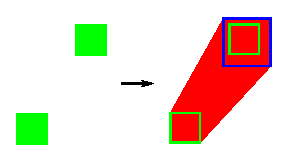
\includegraphics[width=0.45\columnwidth]{images/flowpipe.eps}
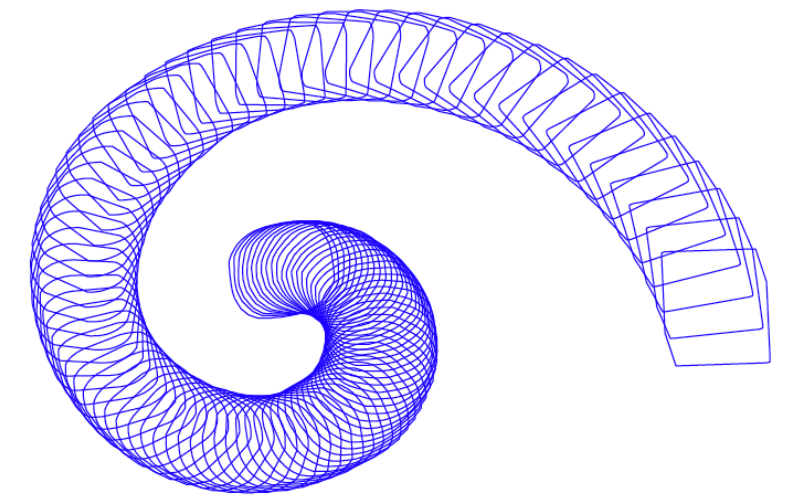
\includegraphics[width=0.45\columnwidth]{images/zono.png}
\caption{On the left: an example of the construction of a containing set for all the possible values between two sets obtained by analytic solving (in green). First bloat one of the sets (in blue), then take the convex hull of the resulting sets (in red). On the right: an example of a flowpipe.}
\label{fowpipeconstruction}
\end{figure}

There exists different sub-methods for the flowpipe construction, each corresponding to different methods to describe the sets of the possible values of the variables. Zonotopes (right part of Figure~\ref{fowpipeconstruction} - the flowpipe is created by zonotopes), support functions and boxes are examples of state set representations. Several operations have to be performed on these sets during flowpipe computation, for instance intersections to detect a collision with a forbidden state. How these set are described in the machine has a strong influence on the computational effort required to perform different operations on the respective set. The internship is about a method to switch between two representations of polyhedra: the $\mathcal{V}$ representation and the $\mathcal{H}$ representation according to Theorem~\ref{thm_representation}.% First some notations and definitions for the rest of the paper:
 

Notations used throughout the paper, the problem is studied in $\mathbb{R}^d$, $d\in \mathbb{N}$:
\begin{itemize}
	\item $conv(V)$ defines the convex hull of the set of vertices $V$: $\{ x\in\mathbb{R}^d| x=\sum_{v\in V} \lambda_v v, \sum_{v\in V} \lambda_v =1, \forall v \in V, \ 0\leq \lambda_v \in \mathbb{R} \}$.
	\item $cone(C)$ defines the conic hull of the vectors in $C$: $\{ x\in\mathbb{R}^d| x=\sum_{c\in C} \lambda_c c, \forall c \in C,\ 0\leq \lambda_c \in \mathbb{R} \}$.
	\item $lineal(L)$ is the linear space generated by $L$: $\{ x\in\mathbb{R}^d| x=\sum_{l\in L} \lambda_l l, \forall l \in L,\ \lambda_l \in \mathbb{R} \}$. For $L$ a set of vectors, $lineal(L)$ is a linealty space. 
	\item In the paper, a sum between two sets is the Minkowsky sum: $S_1+S_2=\{s_1+s_2|s_1\in S_1,\ s_2 \in S_2 \}$.
	\item A half-space $h$ is an area of $\mathbb{R}^d$ defined by a normal vector $a$ and a constant $b$, $h=\{x\in\mathbb{R}^d|x\cdot a\leq b\}$, its border is the hyperplane $\{x\in\mathbb{R}^d|x\cdot a = b\}$. A family of half-spaces are said independent if their normal vectors are independent. Independent hyperplanes are defined respectively. $d$ independent hyperplanes intersect in a vertex.
	\item Let $A$ be a $(n\times d)$-matrix which rows are normal vectors of a finite set of $n$ half-spaces and $b$ the $n$-column vector composed by the corresponding constants. $P(A,b)=\{x\in\mathbb{R}^d|Ax\leq b\}$ is the set of the points contained in all the half-spaces.
	\item An $\mathcal{H}$-polyhedron $P$ is the intersection of a given finite set of half-spaces. There exist $n\in \mathbb{N}$, $A$ a $(n\times d)$-matrix and $b$ a $n$-column vector such that $P=P(A,b)$.
	\item A $\mathcal{V}$-polyhedron $P$ is the Minkowsky sum (from now on refereed as sum) of the convex hull of a finite set of points and a conic hull of a finite set of points, $P=conv(V)+cone(C)$ for some finite $V$ and $C$.
	\item A polyhedron is an $\mathcal{H}$-polyhedron or a $\mathcal{V}$-polyhedron.
	\item A polytope is a bounded polyhedron (and respectively with $\mathcal{H}$ and $\mathcal{V}$-polytopes).
\end{itemize}
 

\begin{theorem}[Polyhedra representation]
A Subset $P\subseteq\mathbb{R}^d$ is an $\mathcal{H}$-polyhedron if and only if it is a $\mathcal{V}$-polyhedron \cite{ziegler_polytopes}.
\label{thm_representation}
\end{theorem} 

\begin{figure}
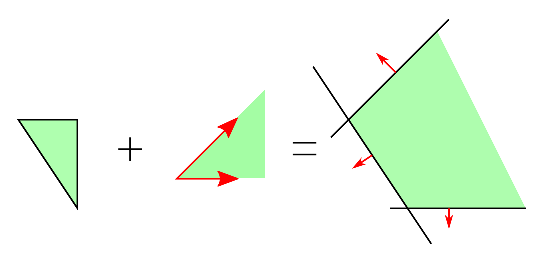
\includegraphics[scale=1]{images/poly.eps}
\caption{Illustration of Theorem~\ref{thm_representation}. From left to right: the sum of the convex hull of a set of vertices and a cone equals an intersection of half-spaces.}
\end{figure}

These two representations have their own advantages and disadvantages, which are summed up  in Tableau~\ref{comparison tab}. As the computational effort for most operations is complementary, being able to switch between both representations is crucial.

\begin{table}
\begin{tabular}{| c | c | c | c |}
	\hline	
				    & $.\ \cap\ .$ & $.\ \cup\ .$ & $.\ +\ .$ \\ \hline
	$\mathcal{V}$-Polyhedra   & \textcolor{red}{difficult} & \textcolor{green}{easy} & \textcolor{green}{easy} \\ \hline
   	$\mathcal{H}$-Polyhedra   & \textcolor{green}{easy} & \textcolor{red}{difficult} & \textcolor{red}{difficult}\\ \hline
\end{tabular}
\caption{Comparison of the cost of different operations between the two representation of the polyhedra.}
\label{comparison tab}
\end{table}

The hosting research group develops, in the context of the HyPro project, an open-source stand-alone C++ library for the most relevant geometric state set representations: covering boxes, polytopes, zonotopes and support functions. 
The library allows the combination of different representations and over-approximative conversion between them. Regarding polyhedra, it covers conversion between bounded $\mathcal{V}$ and $\mathcal{H}$-Polyhedra, the objective of the internship is to expand the library with the conversion between unbounded polyhedra.

The method developed in this paper and the library is an extension of a method for to convert $\mathcal{H}$-polytopes into $\mathcal{V}$-polytopes. This method was not implemented in HyPro, its implementation is a part of the contribution.

Section~\ref{section_sota} presents the state of the art along with the main algorithm used in this paper: Fukuda's algorithm. Section~\ref{section_contrib} contains the contribution of the internship. This reports ends with a conclusion summing up the presented content in Section~\ref{section_conclusion}. 



